% =========================================================================
% Figura: Ejemplos de moléculas aleatorias del conjunto MOSES y sus SMILES
% Disposición minimalista y limpia en 2 filas x 3 columnas
% =========================================================================

\begin{figure}[htbp]
\centering
% Fila 1
\begin{subfigure}[b]{0.32\linewidth}
    \centering
    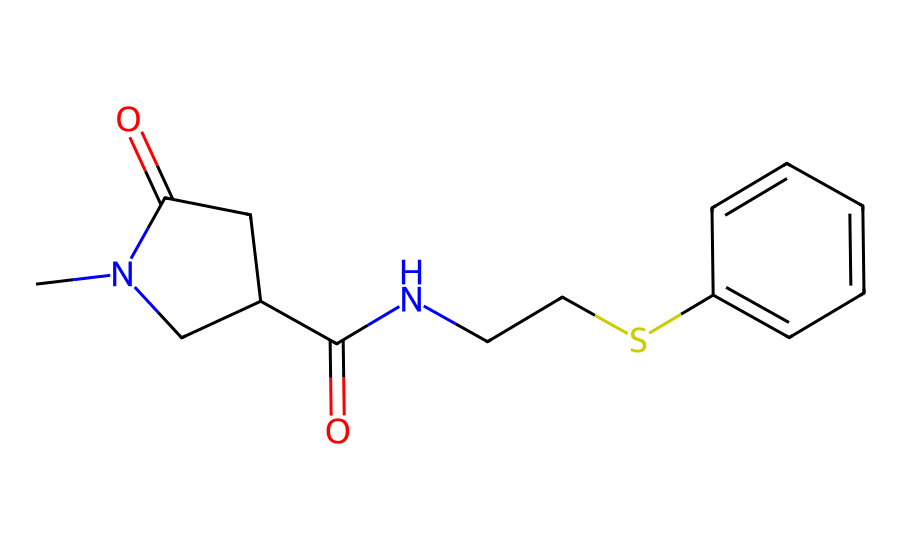
\includegraphics[width=\linewidth, height=2.2cm, keepaspectratio]{Figures/moses_samples/moses_mol_1.png}\par\vspace{3pt}
    {\fontsize{6.2}{7.5}\selectfont\ttfamily CN1CC(C(=O)NCCSc2ccccc2)CC1=O}
\end{subfigure}\hfill
\begin{subfigure}[b]{0.32\linewidth}
    \centering
    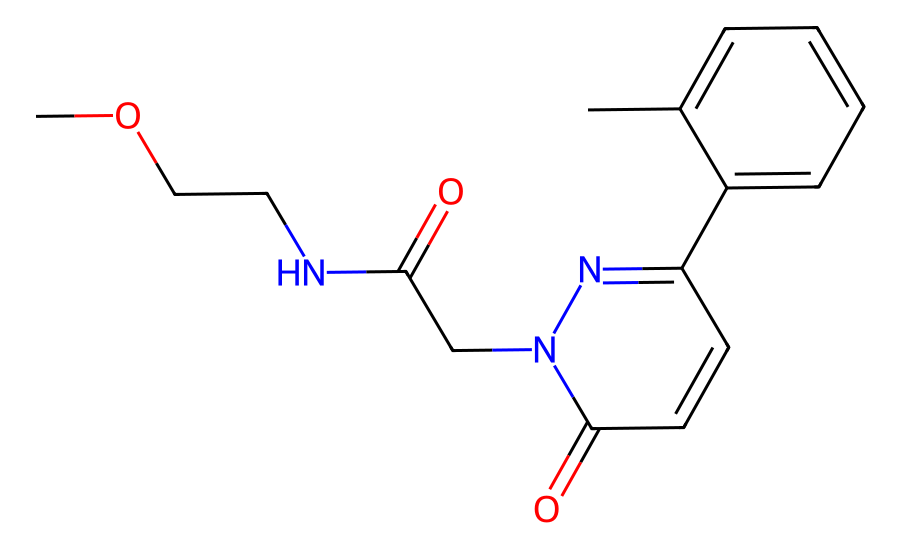
\includegraphics[width=\linewidth, height=2.2cm, keepaspectratio]{Figures/moses_samples/moses_mol_2.png}\par\vspace{3pt}
    {\fontsize{6.2}{7.5}\selectfont\ttfamily COCCNC(=O)Cn1nc(-c2ccccc2C)ccc1=O}
\end{subfigure}\hfill
\begin{subfigure}[b]{0.32\linewidth}
    \centering
    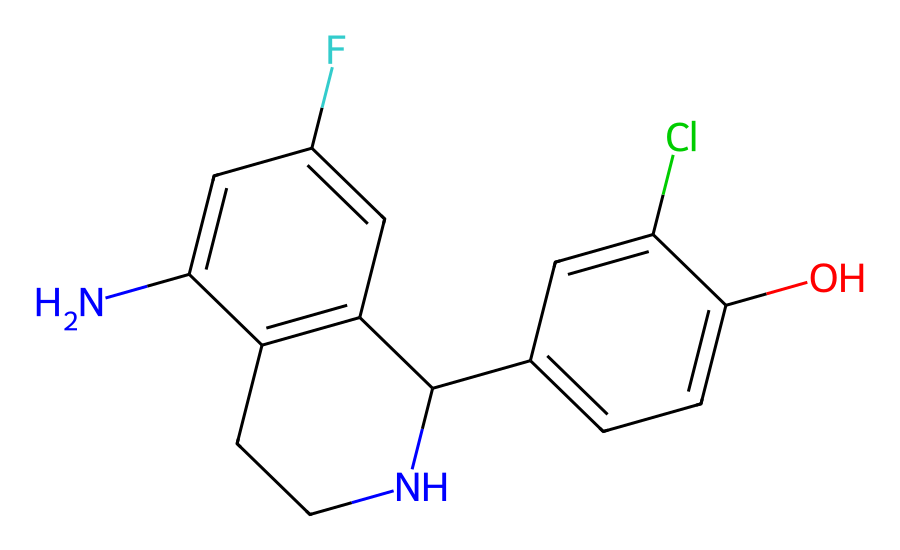
\includegraphics[width=\linewidth, height=2.2cm, keepaspectratio]{Figures/moses_samples/moses_mol_3.png}\par\vspace{3pt}
    {\fontsize{6.2}{7.5}\selectfont\ttfamily Nc1cc(F)cc2c1CCNC2c1ccc(O)c(Cl)c1}
\end{subfigure}

\vspace{10pt}

% Fila 2
\begin{subfigure}[b]{0.32\linewidth}
    \centering
    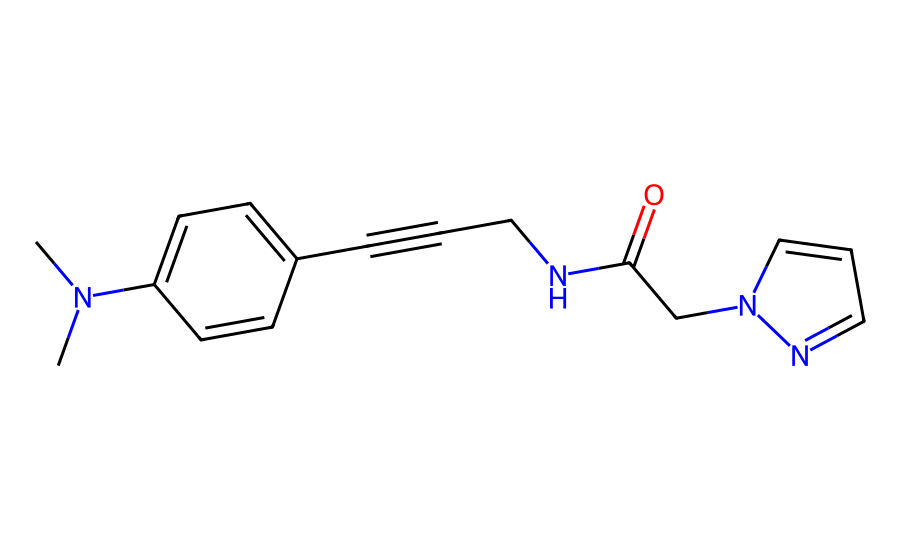
\includegraphics[width=\linewidth, height=2.2cm, keepaspectratio]{Figures/moses_samples/moses_mol_4.png}\par\vspace{3pt}
    {\fontsize{6.2}{7.5}\selectfont\ttfamily CN(C)c1ccc(C\#CCNC(=O)Cn2cccn2)cc1}
\end{subfigure}\hfill
\begin{subfigure}[b]{0.32\linewidth}
    \centering
    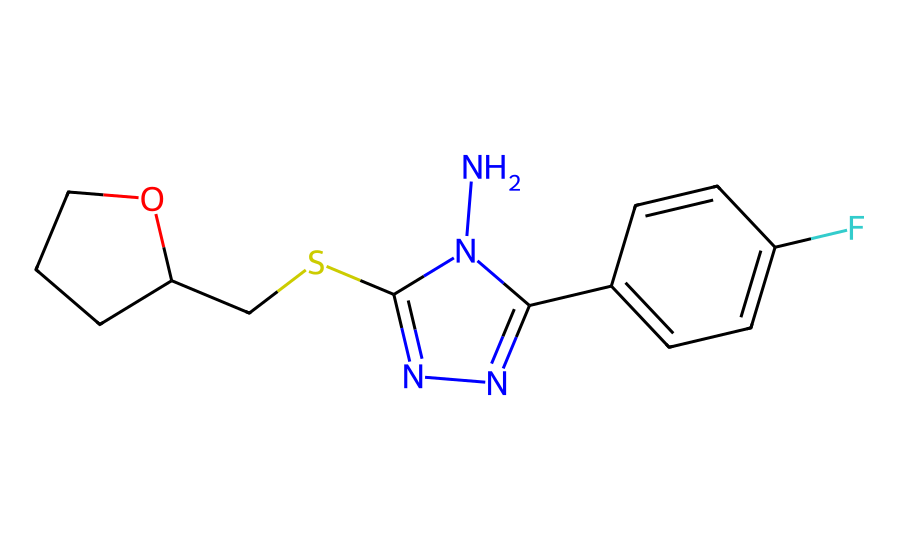
\includegraphics[width=\linewidth, height=2.2cm, keepaspectratio]{Figures/moses_samples/moses_mol_5.png}\par\vspace{3pt}
    {\fontsize{6.2}{7.5}\selectfont\ttfamily Nn1c(SCC2CCCO2)nnc1-c1ccc(F)cc1}
\end{subfigure}\hfill
\begin{subfigure}[b]{0.32\linewidth}
    \centering
    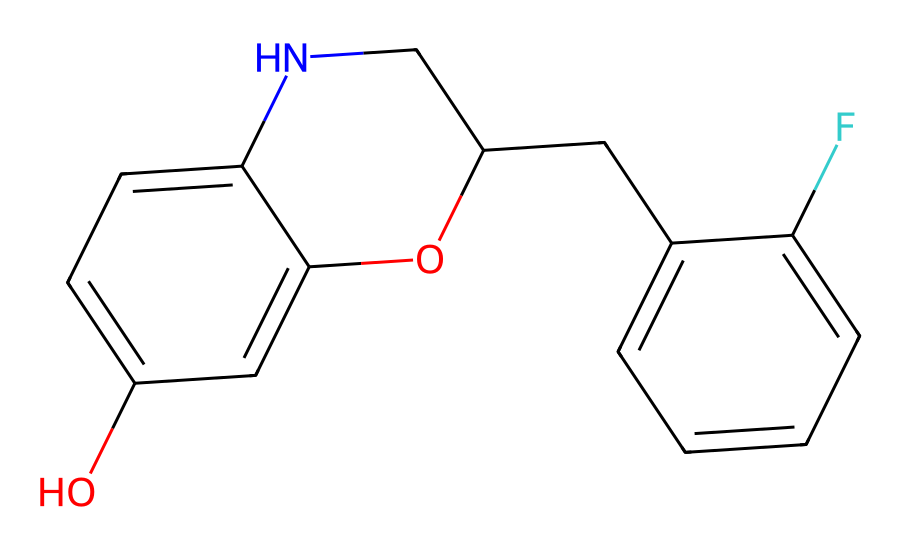
\includegraphics[width=\linewidth, height=2.2cm, keepaspectratio]{Figures/moses_samples/moses_mol_6.png}\par\vspace{3pt}
    {\fontsize{6.2}{7.5}\selectfont\ttfamily Oc1ccc2c(c1)OC(Cc1ccccc1F)CN2}
\end{subfigure}

\vspace{6pt}
\caption{Ejemplos de moléculas del conjunto de datos MOSES y su correspondiente representación lineal en formato SMILES.}
\label{fig:muestras_moses}
\end{figure}
